% CMP6200 / DIG6200 — Final Progress Review
% Aligned with Interim_Report.pdf §3.2 objectives
% Tables and listings are included as images from figures/
% Build: ./build.sh
\documentclass[11pt,a4paper]{article}
\usepackage[margin=2.5cm]{geometry}
\usepackage{graphicx}
\usepackage{natbib}
\linespread{1.5}\selectfont
\setlength{\parindent}{0pt}
\setlength{\parskip}{0.4em}

\begin{document}

\begin{titlepage}
\centering
\vspace*{1.2cm}
{\large CMP6200 / DIG6200}\\[0.3em]
{\large Individual Undergraduate Project (FYP)}\\[1em]
{\LARGE\textbf{Final Progress Review}}\\[0.8em]
{\large\textbf{Real-Time Context-Aware Sign Language to Multilingual Speech}}\\
{\large\textbf{Conversion System with Emotion Detection}}\\[0.4em]
{\normalsize Hybrid recognition, T5 NLP, emotion prosody and Nepali TTS}\\[1.5em]
{\large Student Name: Kevin Raj Karki \quad Student ID: 23189623}\\[0.3em]
{\large Course: BSc (Hons) Computing}\\[0.3em]
{\large Supervisor: Manoj Gautam}\\[1.2em]
{\large Reporting Period: April 2026 (interim report) to August 2026}
\vfill
\end{titlepage}

\newpage
\tableofcontents
\newpage

\section{1.0 Progress to Date --- Summary}

The project is in advanced implementation and evaluation.
Since the interim report, the React/FastAPI \texttt{ASLPipeline} was completed with Alphabet and WLASL Words modes, then evaluated against all five SMART objectives \citep{li2020wlasl,raffel2020t5}.
Objective~1 is \textbf{partially met}: 50 WLASL glosses and 93.7\% alphabet webcam accuracy after hybrid fine-tuning, but WLASL word accuracy is 60.7\% (below 85\%).
Objectives~2--4 are \textbf{met}: NLP BLEU 19.2$\rightarrow$57.6, gloss-path latency p95 814\,ms, and one webcam-only pipeline.
Objective~5 is \textbf{in progress}: metrics done; SUS awaits ethics approval \citep{brooke1996sus}.
Beyond interim scope excluding facial expressions (Interim Report \S3.3), emotion-aware prosody was added for the project title; live tests detect happy, neutral and angry reliably.

\section{2.0 Artefact Design and Development}

This section presents artefact evidence against the interim design (Interim Report \S4.1--4.2).

\subsection{2.1 Implementation and Current State}

The stack is React $\rightarrow$ FastAPI WebSocket $\rightarrow$ PyTorch/TensorFlow via \texttt{ASLPipeline}: MediaPipe landmarks, Alphabet/WLASL recognition, gloss assembly, T5 or rule-based NLP, facial emotion, and gTTS English/Nepali with emotion prosody.
Figure~\ref{fig:architecture} shows the architecture; Figure~\ref{fig:wlasl_progress} shows WLASL accuracy gains since the interim CNN-LSTM plan.

\begin{figure}[htbp]
\centering
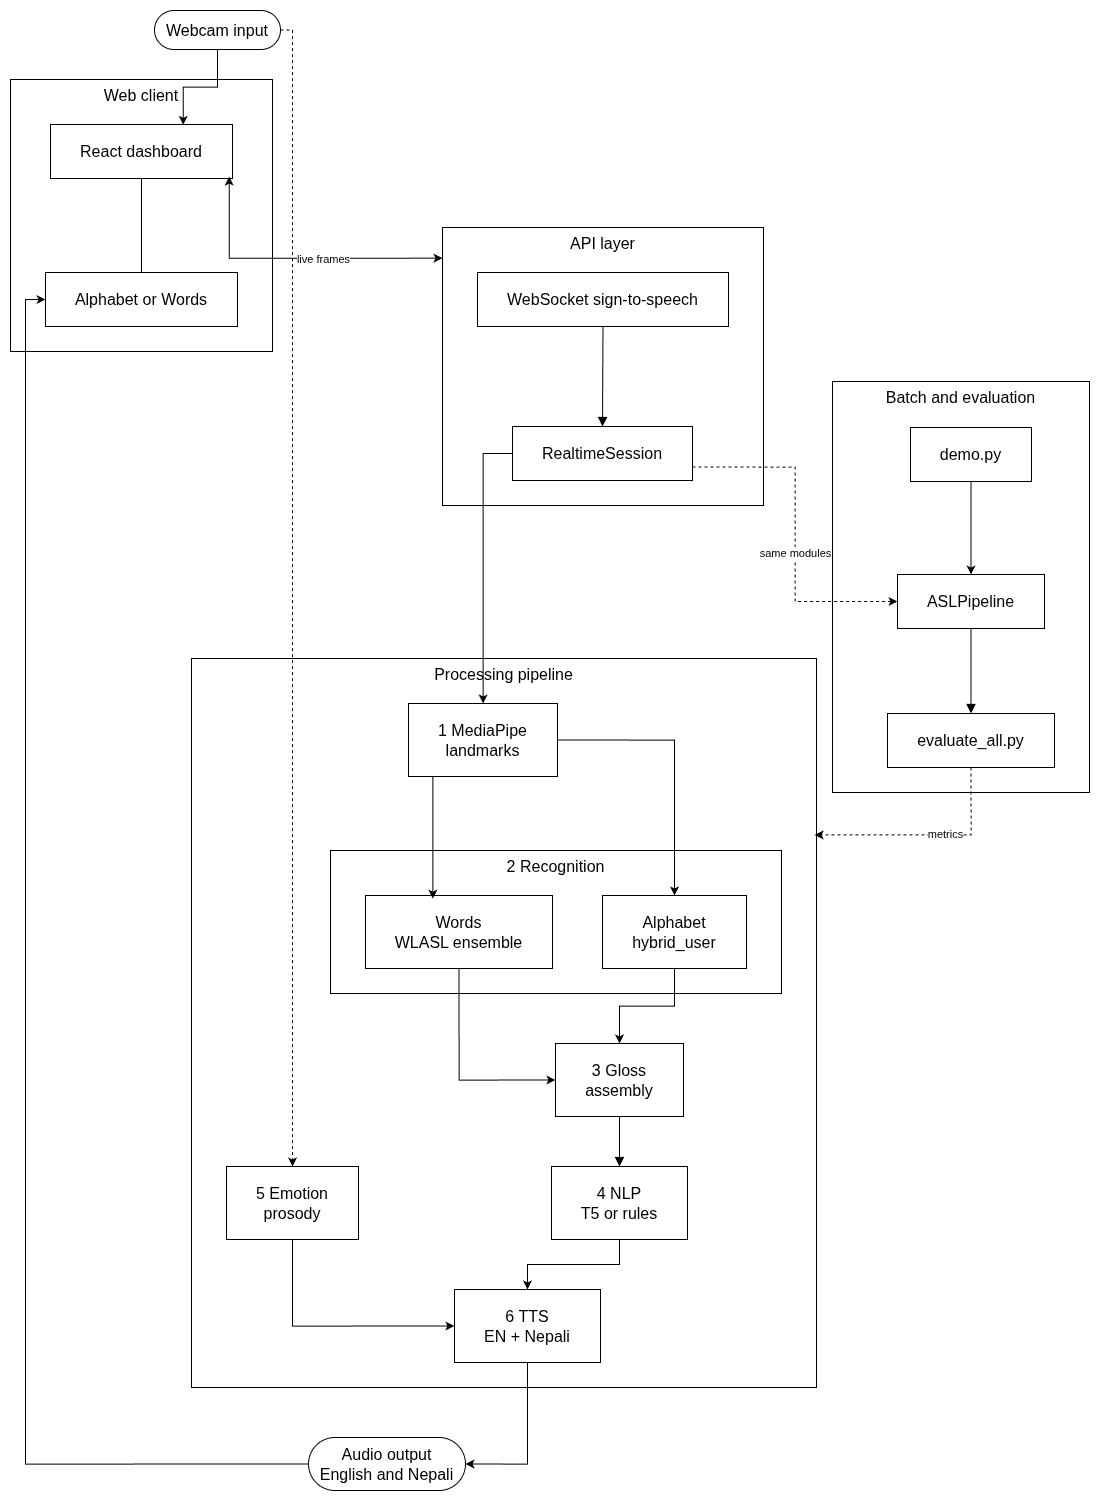
\includegraphics[width=0.92\linewidth,height=0.55\textheight,keepaspectratio]{figures/fyp_architecture.png}
\caption{System architecture: web client, FastAPI session, processing pipeline, and batch evaluation.}
\label{fig:architecture}
\end{figure}

\begin{figure}[htbp]
\centering
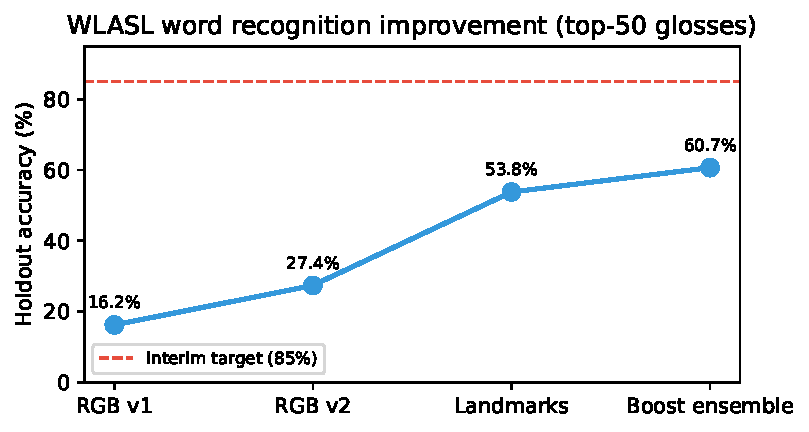
\includegraphics[width=0.72\linewidth]{figures/wlasl_progression.pdf}
\caption{WLASL progression: RGB 27\% $\rightarrow$ landmarks 53.8\% $\rightarrow$ ensemble 60.7\%.}
\label{fig:wlasl_progress}
\end{figure}

Table~\ref{tab:objectives} maps results to Interim Report \S3.2; Figure~\ref{fig:objectives} visualises targets; Table~\ref{tab:challenges} lists key challenges.

\begin{figure}[htbp]
\centering
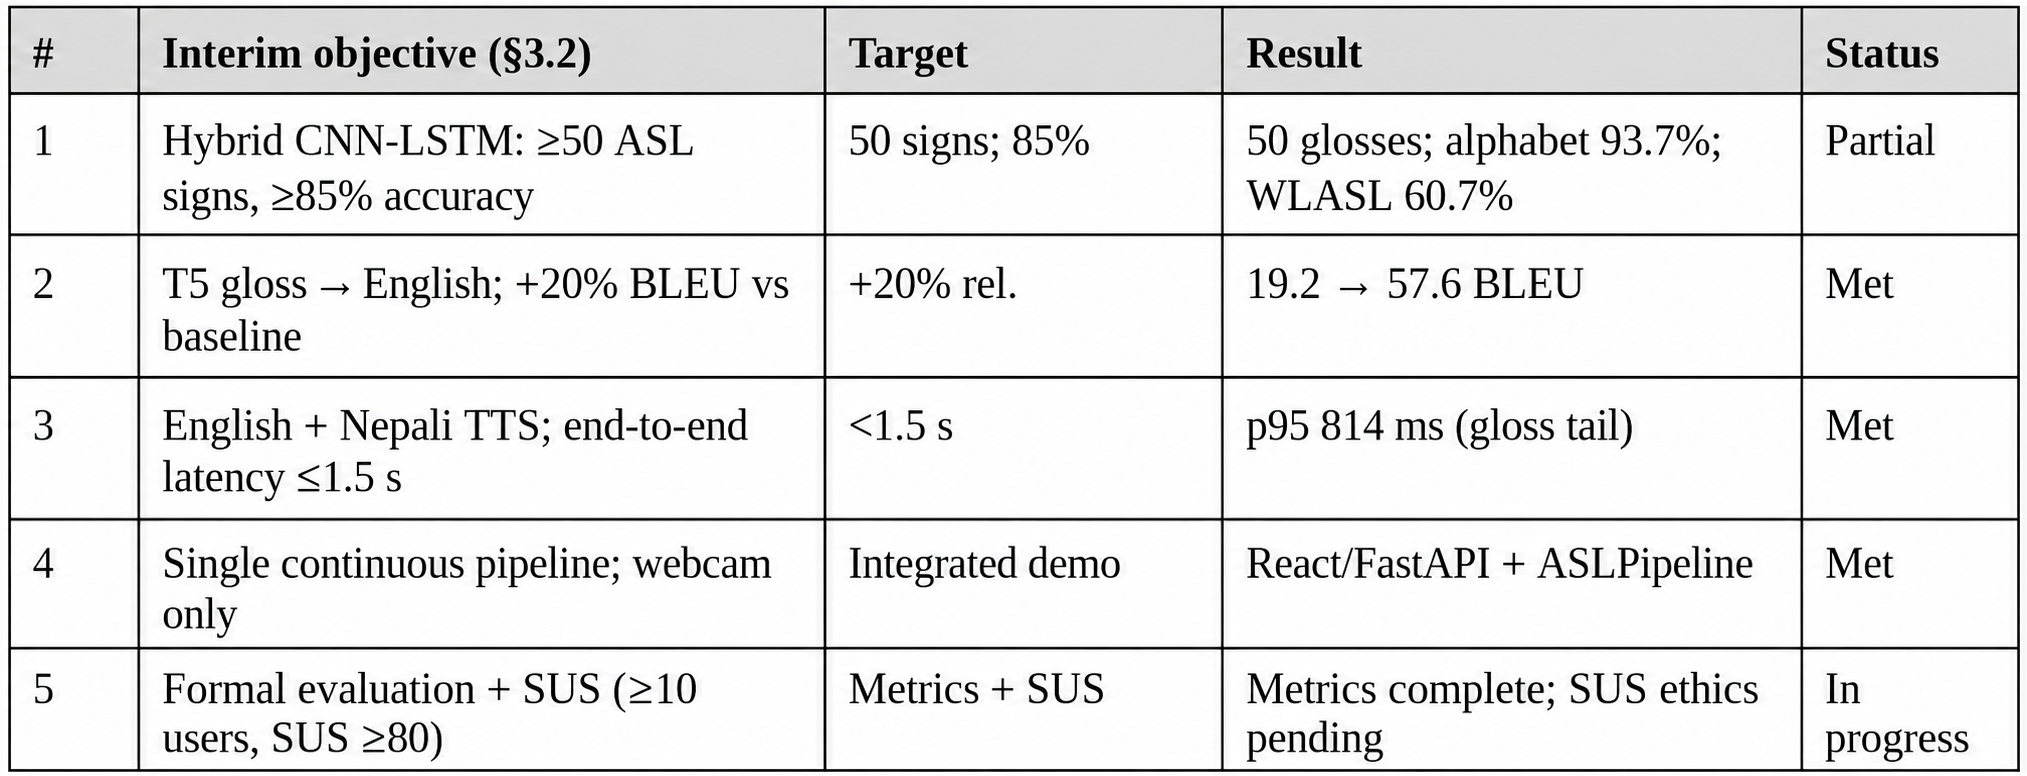
\includegraphics[width=0.98\linewidth]{figures/table_1.png}
\caption{Interim SMART objectives vs results (August 2026).}
\label{tab:objectives}
\end{figure}

\begin{figure}[htbp]
\centering
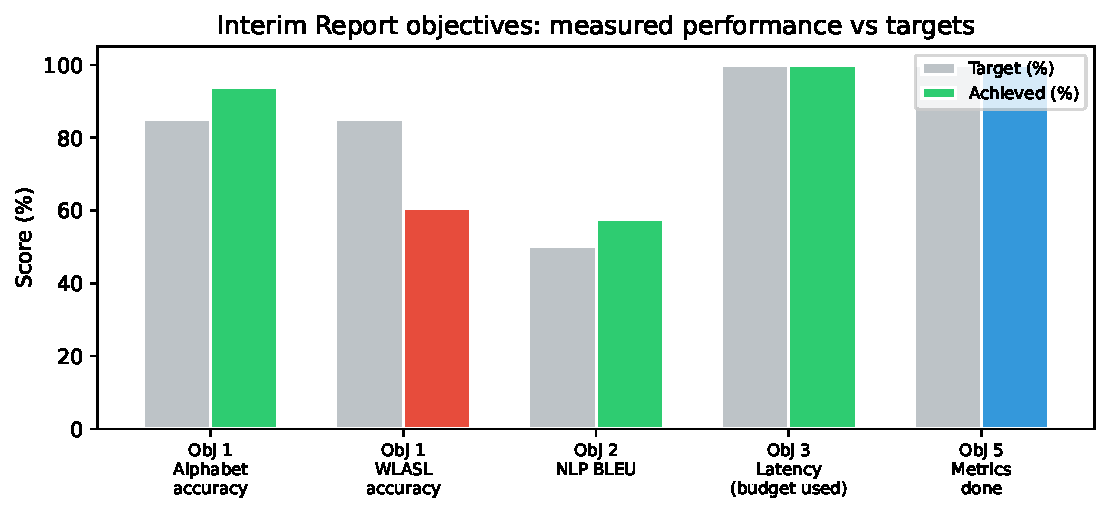
\includegraphics[width=0.82\linewidth]{figures/objectives_comparison.pdf}
\caption{Key metrics against interim targets.}
\label{fig:objectives}
\end{figure}

\begin{figure}[htbp]
\centering
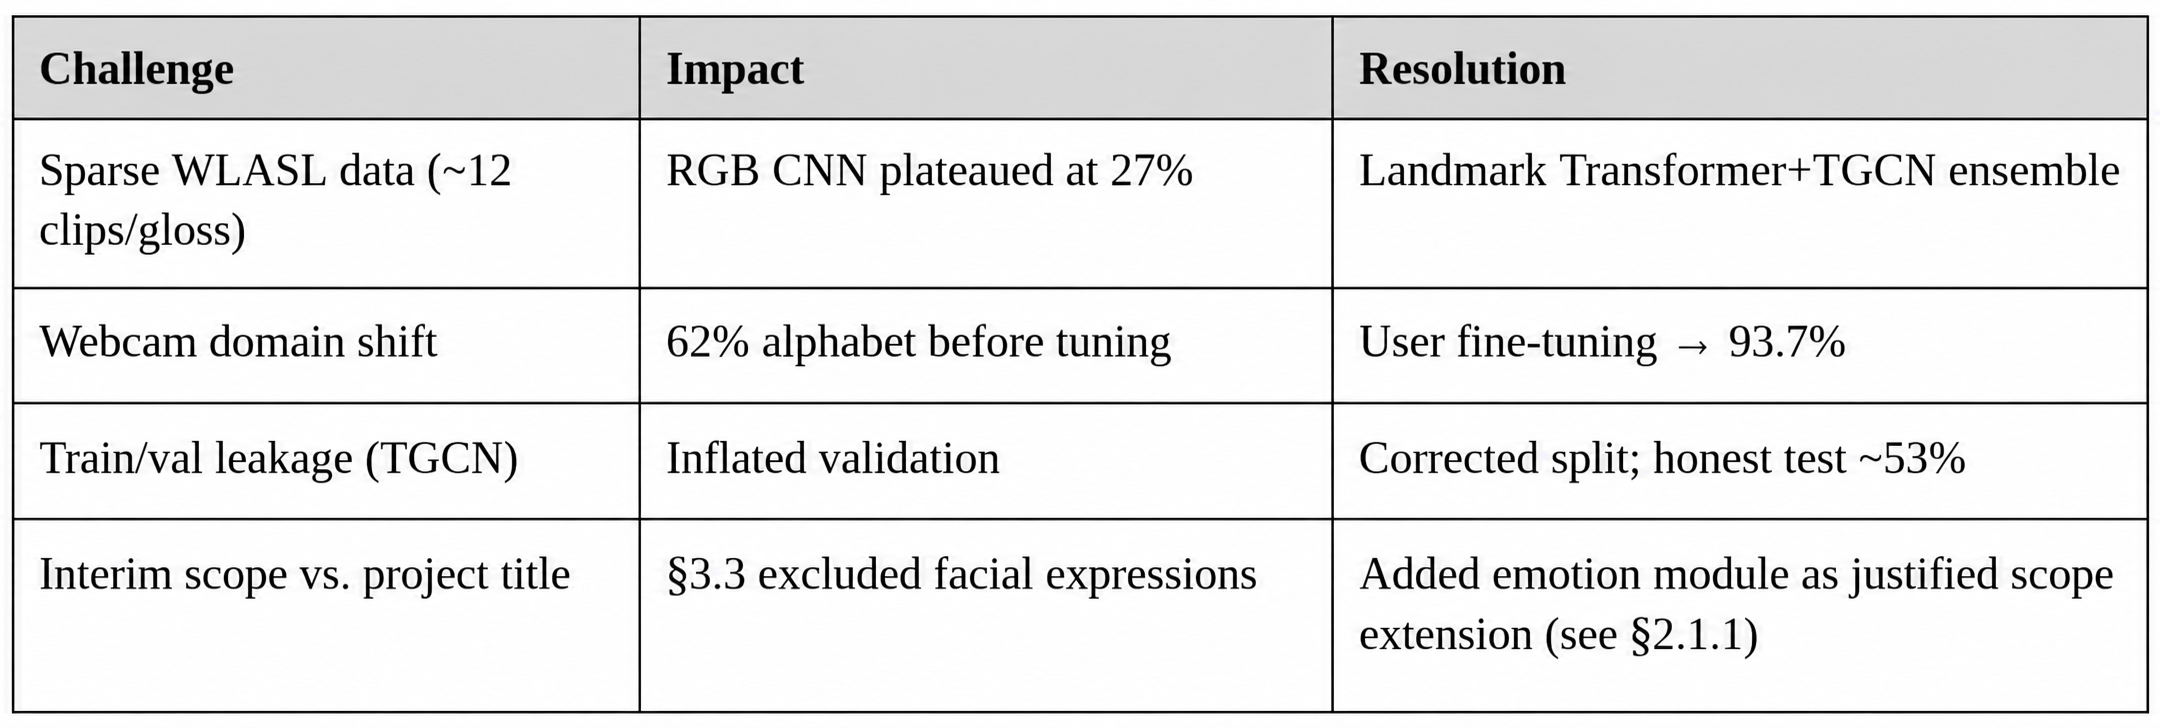
\includegraphics[width=0.98\linewidth]{figures/table_2.png}
\caption{Development challenges and resolutions.}
\label{tab:challenges}
\end{figure}

Figure~\ref{fig:webui} shows Alphabet-mode evidence (sign \textit{V}, 98\% via \texttt{hybrid\_user}).
Figure~\ref{fig:words} shows Words mode with \texttt{wlasl\_landmarks}, clip recording, and Keras emotion status.

\begin{figure}[htbp]
\centering
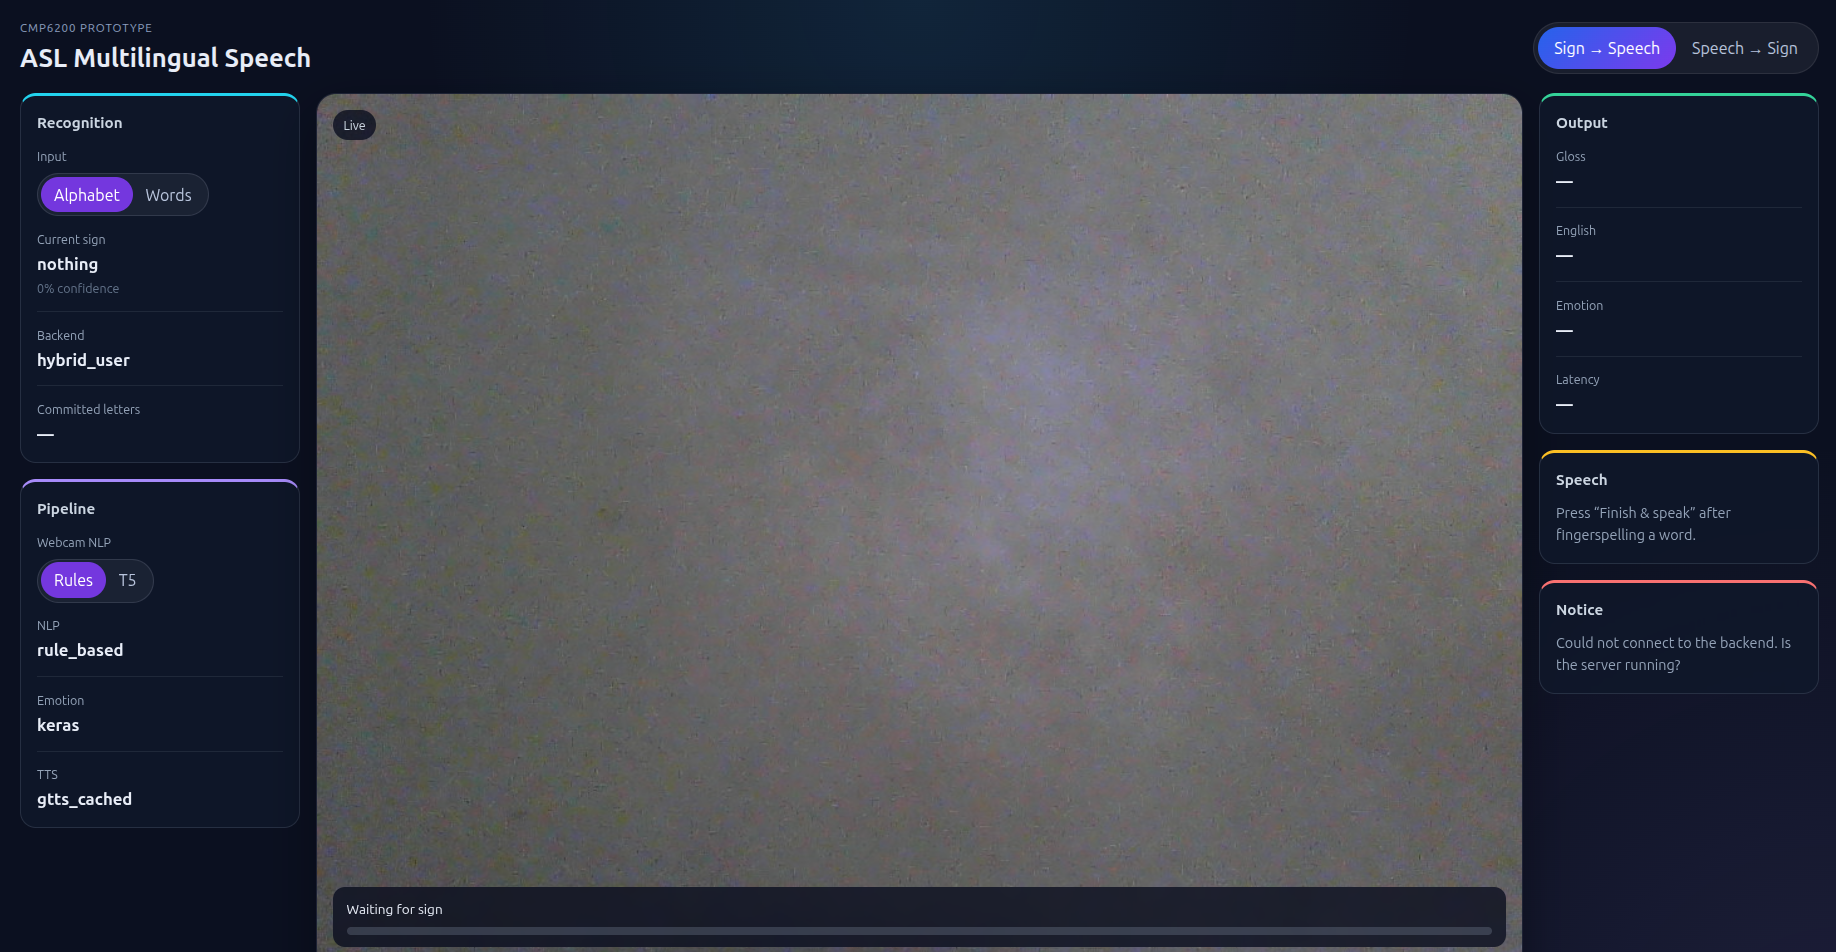
\includegraphics[width=0.48\linewidth]{figures/working_web-app.png}\hfill
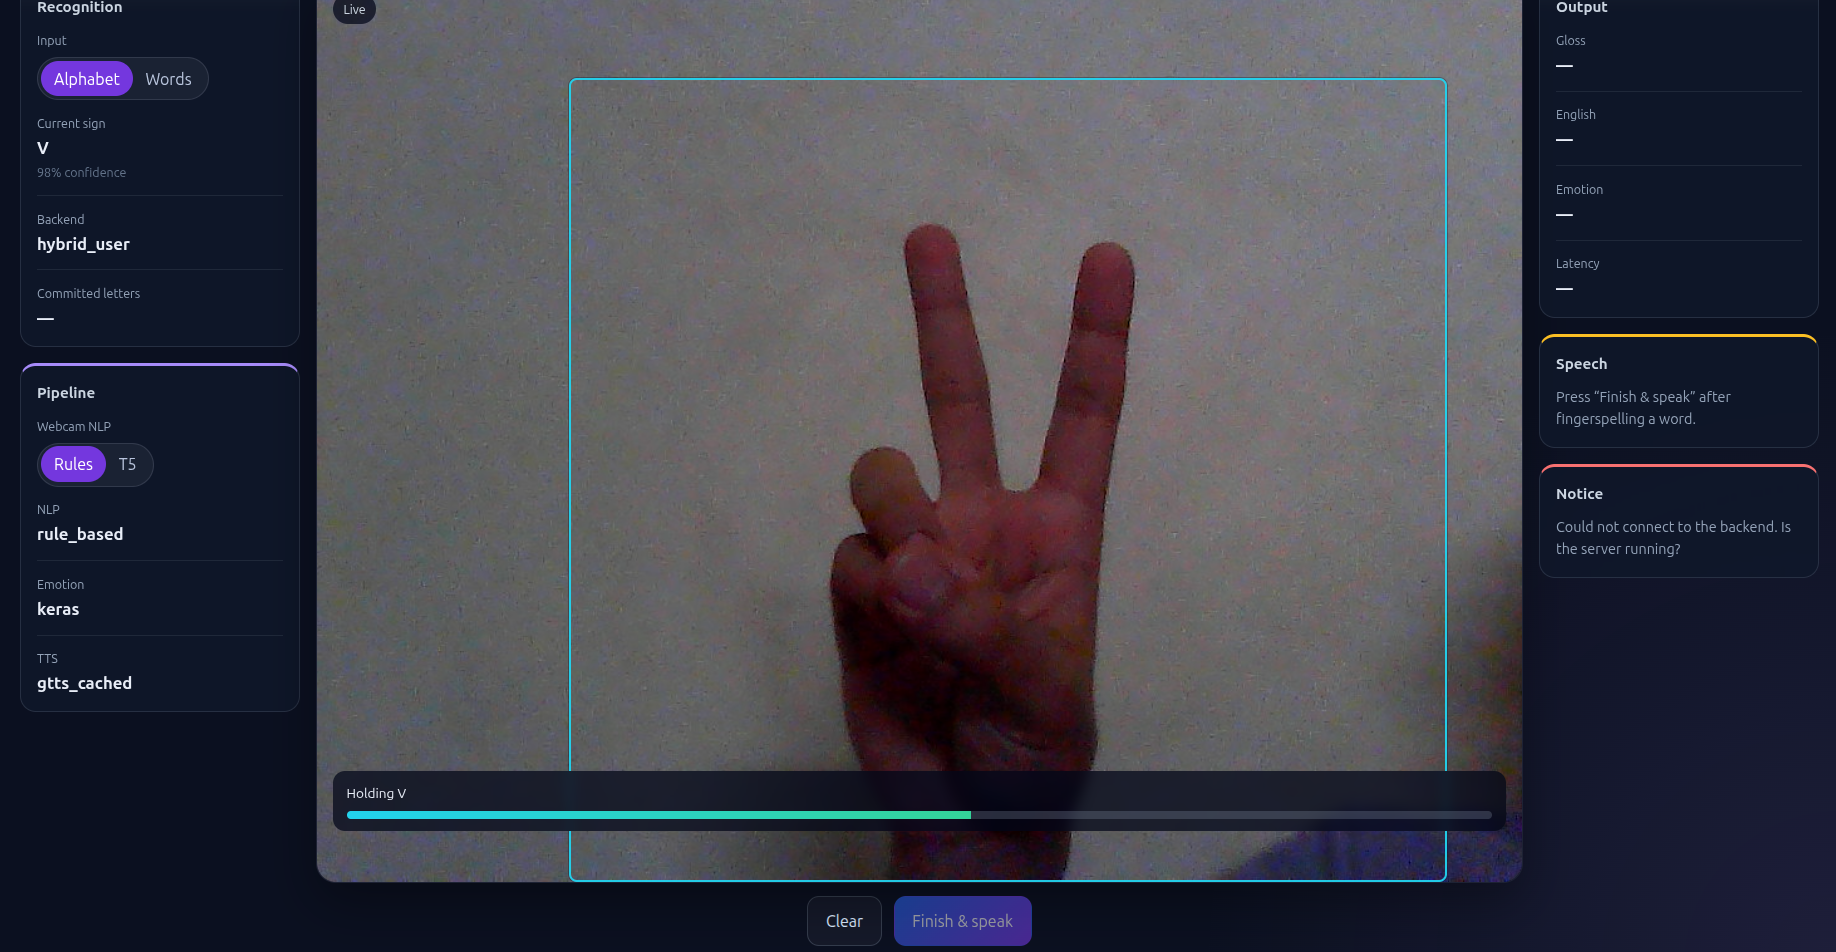
\includegraphics[width=0.48\linewidth]{figures/alphabet-tryon-web-app.png}
\caption{Alphabet mode: dashboard (left) and live try-on (right).}
\label{fig:webui}
\end{figure}

\begin{figure}[htbp]
\centering
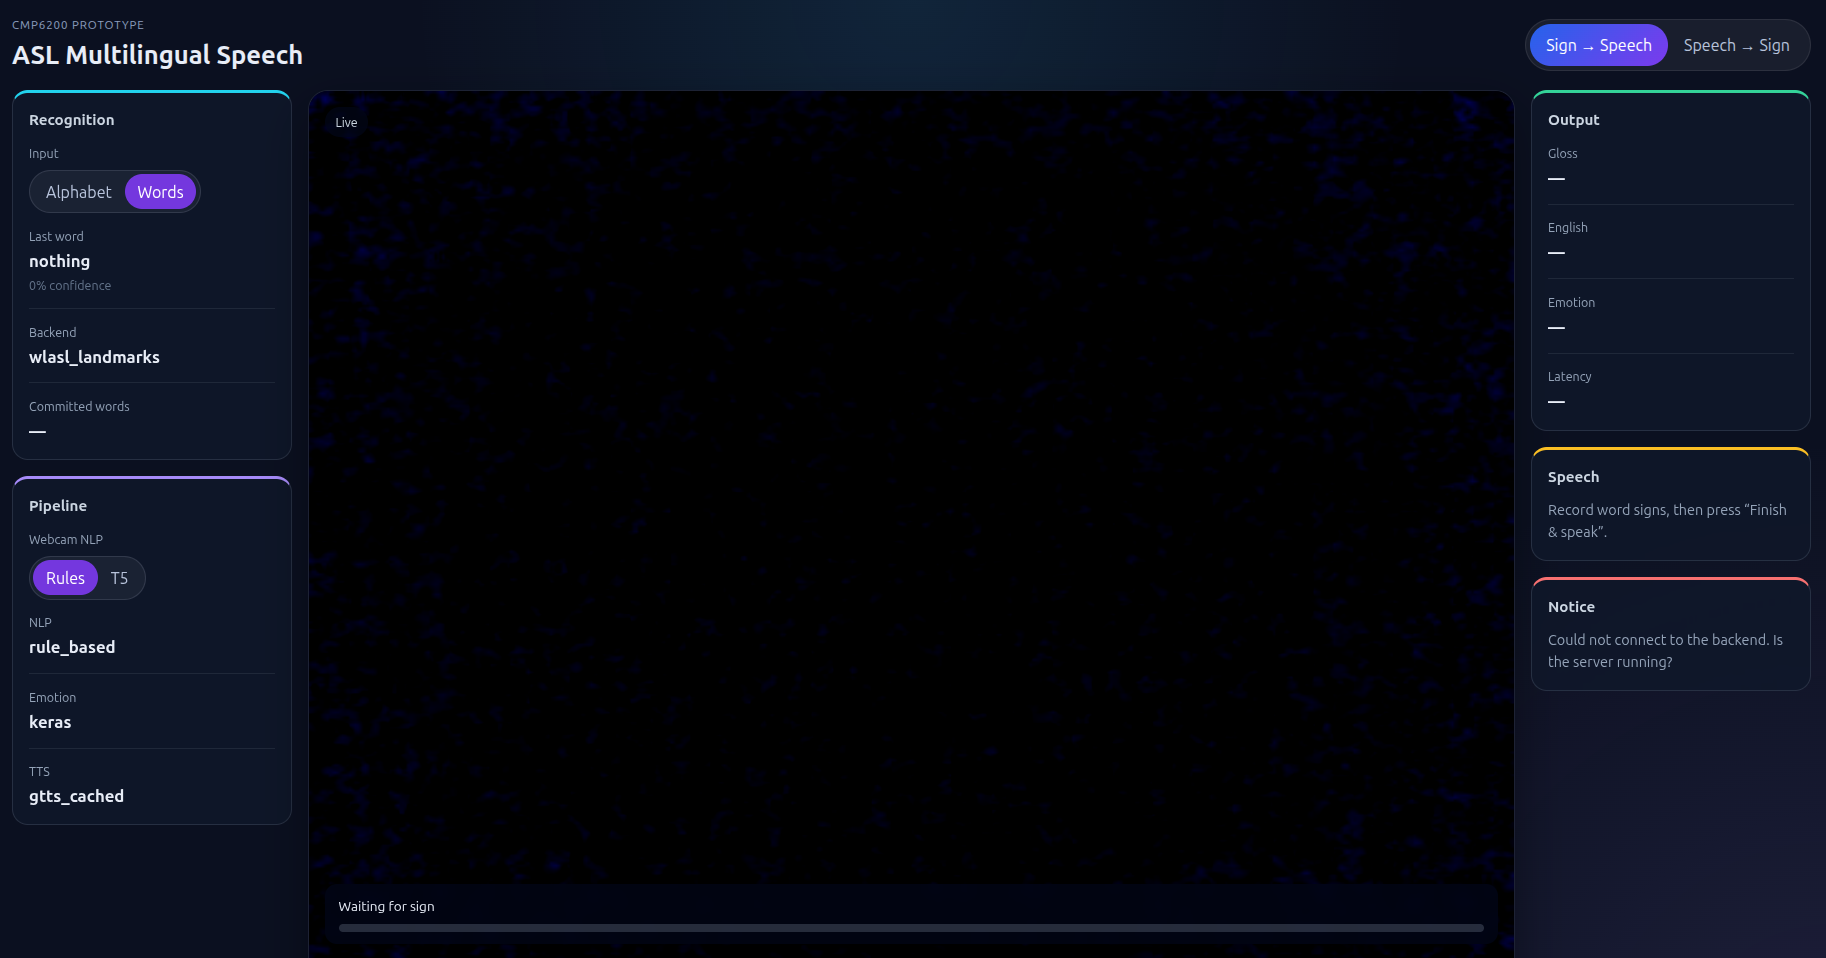
\includegraphics[width=0.90\linewidth]{figures/word_section.png}
\caption{Words (WLASL) mode: clip record, gloss/English/emotion/latency on Finish \& speak.}
\label{fig:words}
\end{figure}

\subsubsection*{2.1.1 Scope extension: emotion-aware prosody}

Interim Report \S3.3 excluded facial expressions, but the project title includes Emotion Detection.
Emotion-aware prosody was therefore added after interim submission so TTS is not monotone \citep{koller2020survey}.

\texttt{EmotionDetector} uses OpenCV Haar face detection, a 48$\times$48 grayscale crop, and a Keras CNN on a four-class FER2013 subset (happy, sad, angry, neutral) \citep{goodfellow2013fer}, mapping emotion to TTS rate/pitch.
Offline accuracy is 65.5\%; live tests reliably detect happy, neutral and angry.
The UI shows the Keras backend and, after Finish \& speak, the emotion label with confidence (e.g.\ happy 0.87).

\begin{figure}[htbp]
\centering
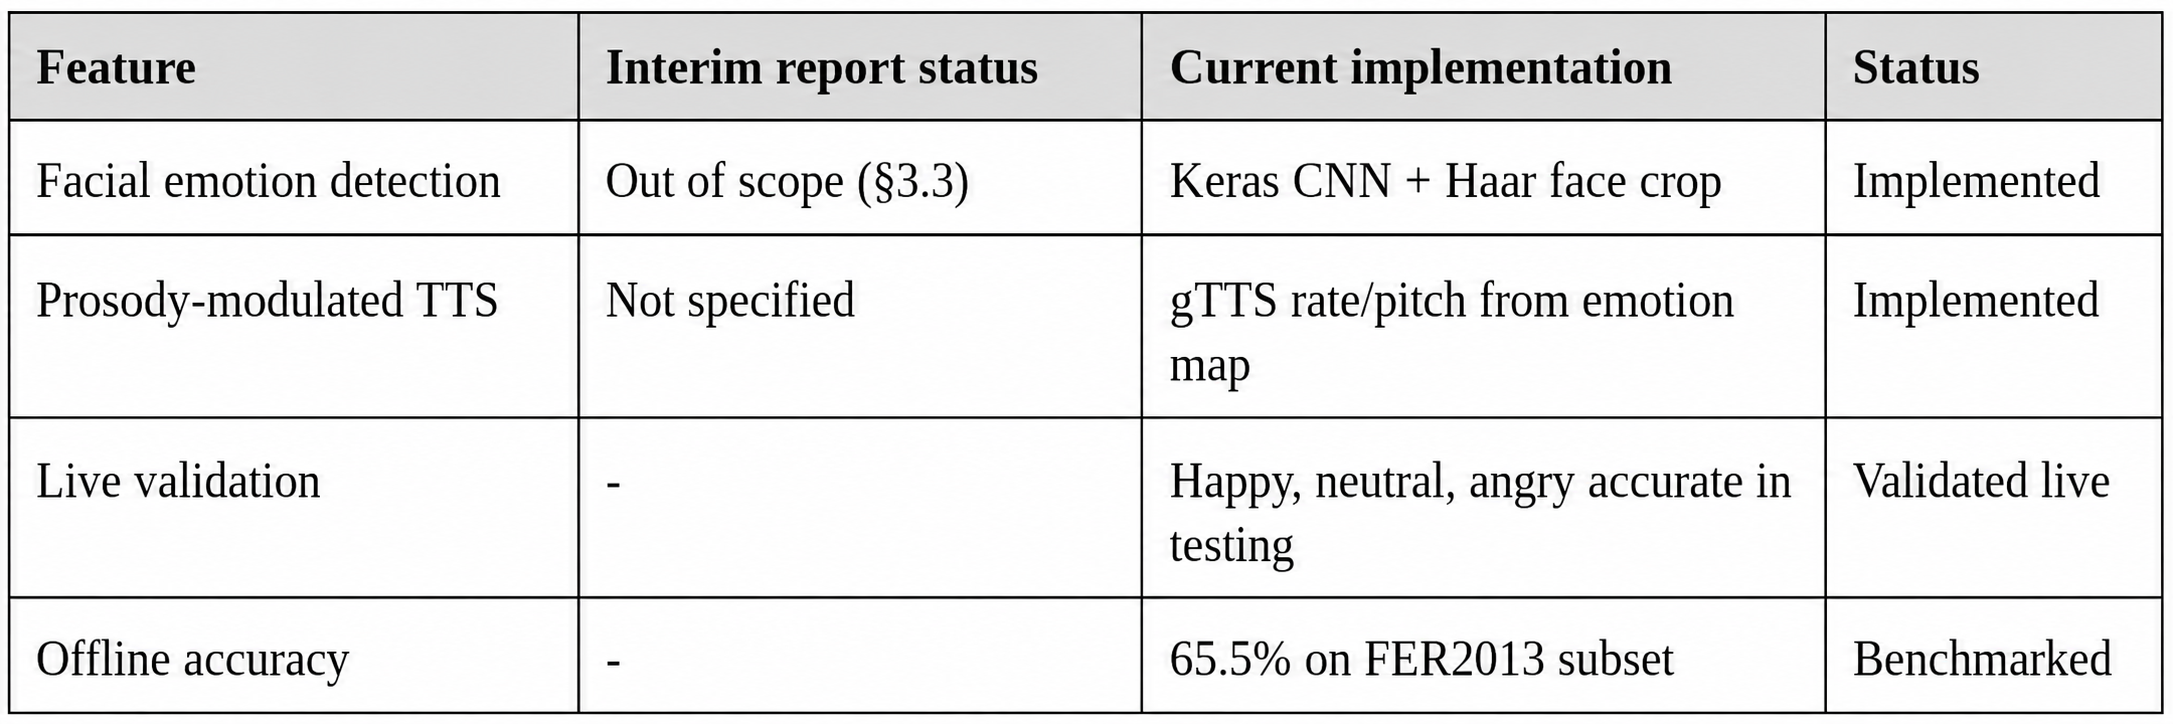
\includegraphics[width=0.98\linewidth]{figures/table_3.png}
\caption{Emotion scope extension (not an interim SMART objective).}
\label{tab:emotion}
\end{figure}

\begin{figure}[htbp]
\centering
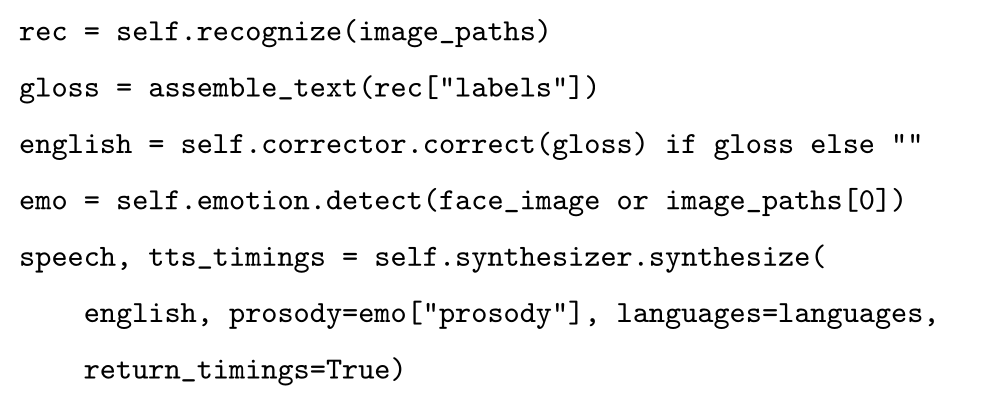
\includegraphics[width=0.95\linewidth]{figures/Listing-1.png}
\caption{Listing 1: Pipeline with emotion (\texttt{pipeline/pipeline.py}).}
\label{lst:pipeline}
\end{figure}

\begin{figure}[htbp]
\centering
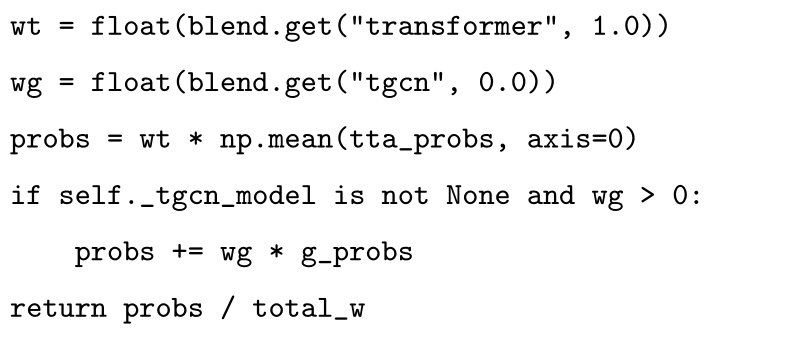
\includegraphics[width=0.95\linewidth]{figures/Listing-2.png}
\caption{Listing 2: WLASL ensemble blend (\texttt{wlasl\_predictor.py}).}
\label{lst:ensemble}
\end{figure}

\subsection{2.2 Analysis and Reflection}

Objectives~2--4 are met; Objective~1 is partial (50 signs met; 85\% met for alphabet only); Objective~5 metrics are done, SUS pending.
Alphabet and WLASL must stay separate for honest Objective~1 reporting.
Emotion is a justified scope extension reconciling Interim Report \S3.3 with the project title.
Skeleton landmarks beat raw-video CNNs on sparse WLASL; user fine-tuning closed the webcam gap.
The main design revision replaced RGB WLASL with a landmark Transformer+TGCN ensemble (Figure~\ref{fig:wlasl_progress}) and added emotion prosody after flat TTS conflicted with the context-aware aim.

\section{3.0 Updated Planning for Project Completion}

The artefact is demo-ready; the critical path is Objective~5 SUS and dissertation writing (Table~\ref{tab:plan}).
\begin{enumerate}\setlength{\itemsep}{1pt}
  \item \textbf{(High)} Ethics-approved SUS ($\geq$10 participants).
  \item \textbf{(High)} Dissertation: interim objectives, emotion extension, separate alphabet/WLASL results.
  \item \textbf{(High)} Demo video (Alphabet, Words, emotion TTS) and viva prep.
  \item \textbf{(Medium)} Document WLASL gap or optional webcam fine-tune as future work.
\end{enumerate}

\begin{figure}[htbp]
\centering
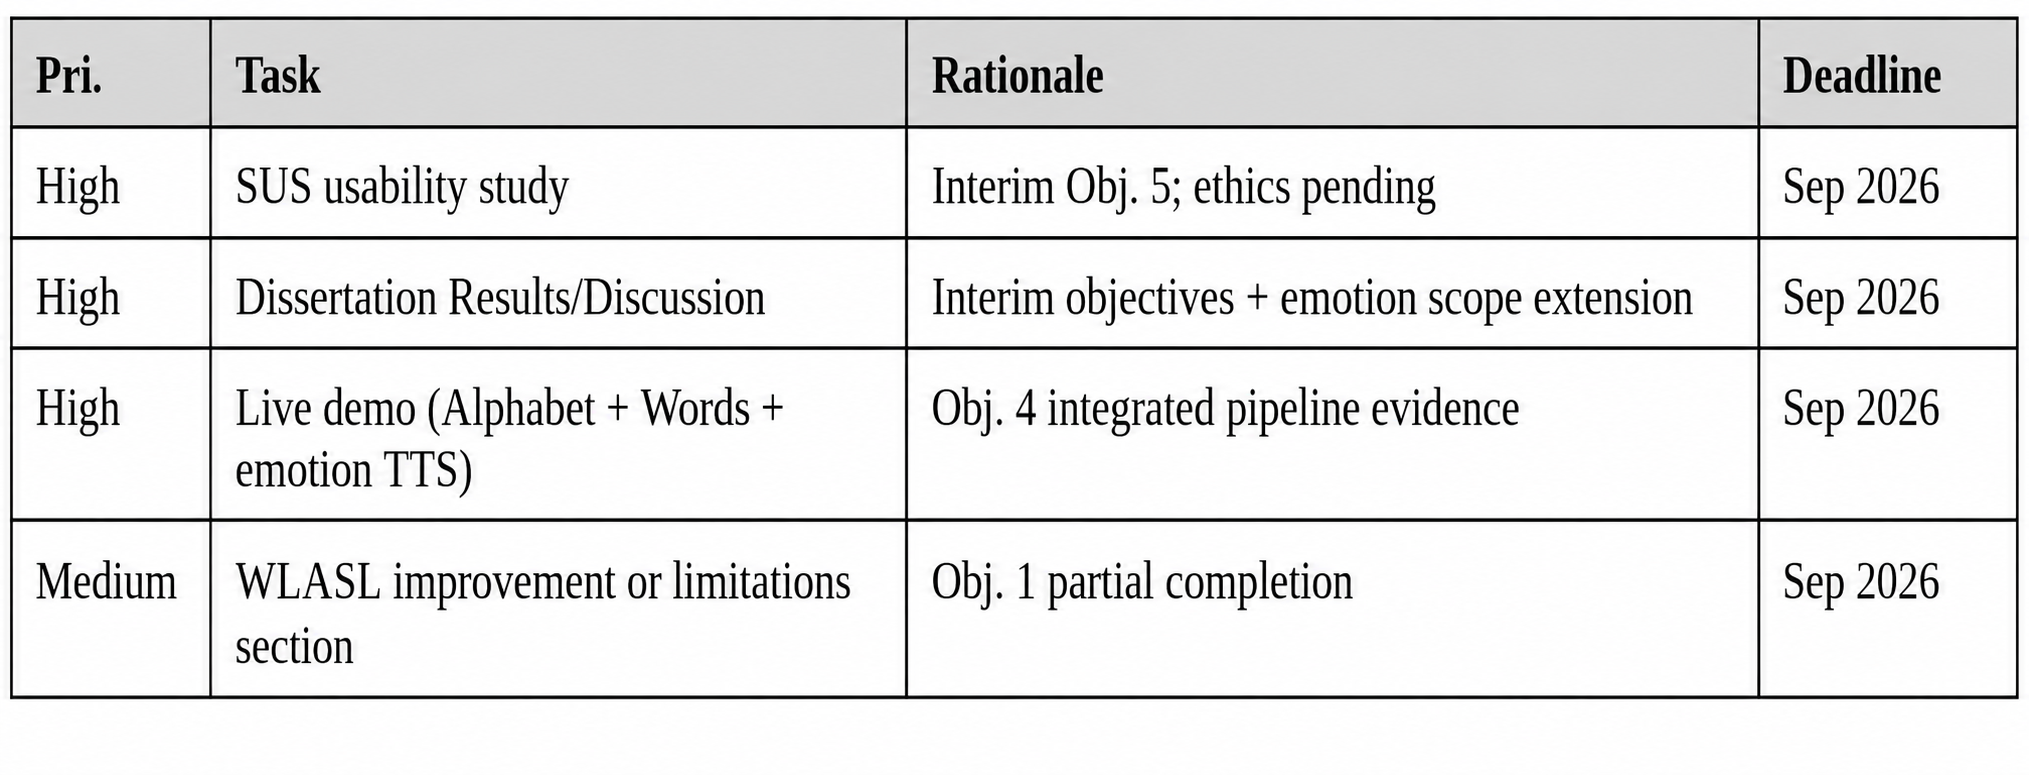
\includegraphics[width=0.98\linewidth]{figures/table_4.png}
\caption{Updated planning (Objective~5 and submission).}
\label{tab:plan}
\end{figure}

\subsection{3.2 Draft Outline of Final Report}

Table~\ref{tab:outline} summarises the dissertation chapter plan.

\begin{figure}[htbp]
\centering
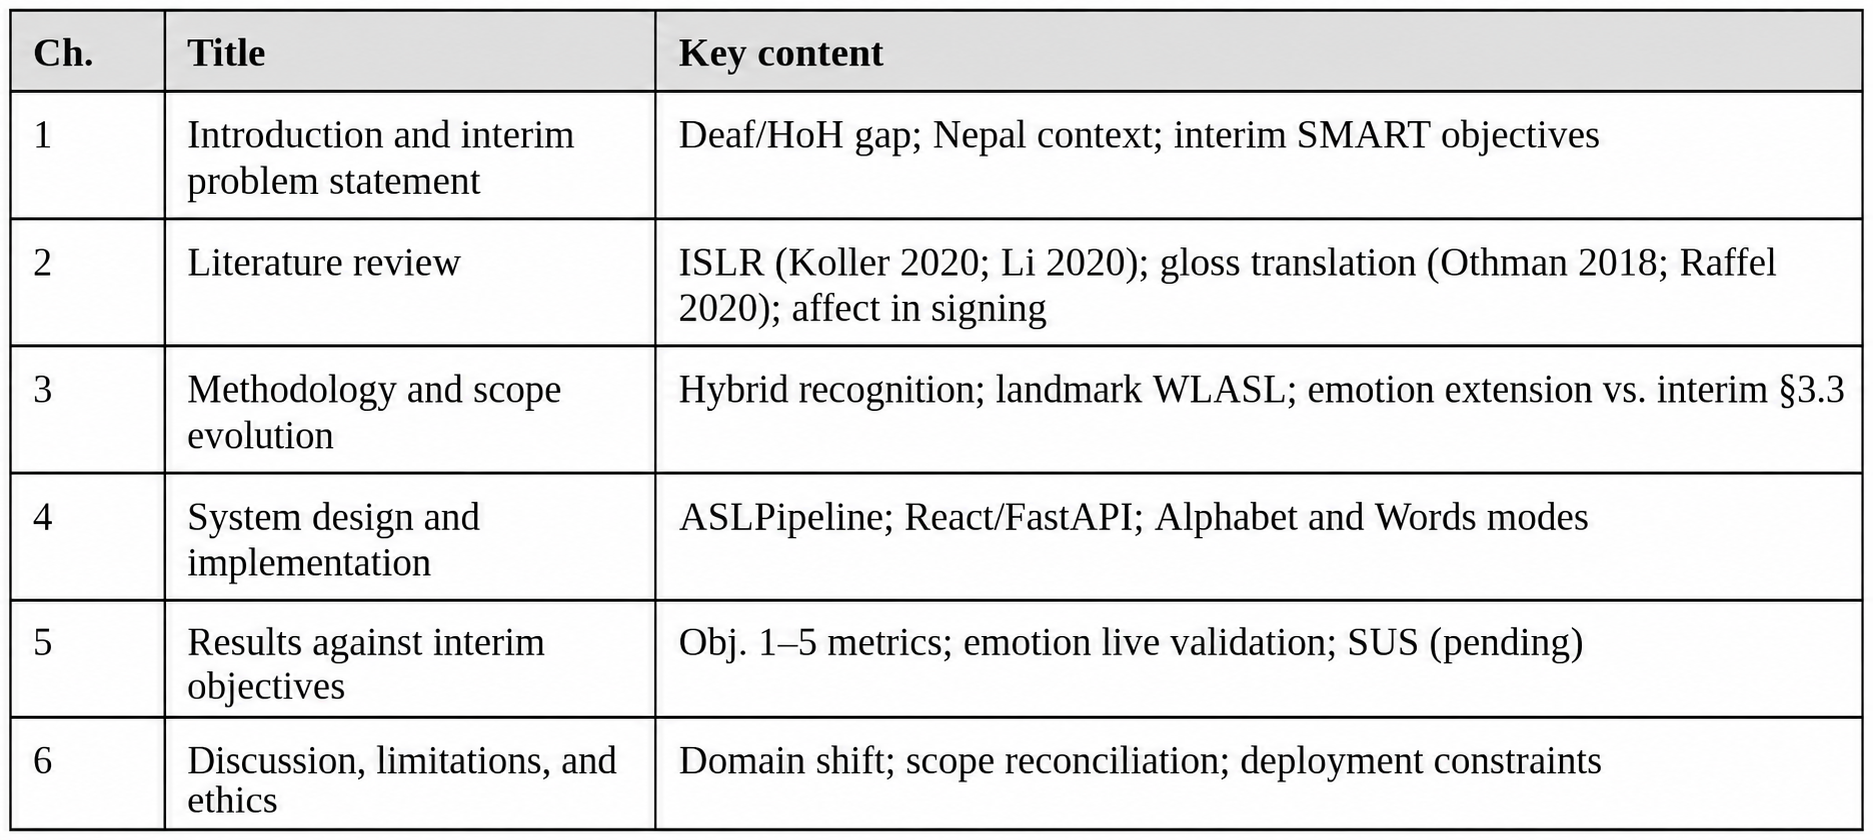
\includegraphics[width=0.98\linewidth]{figures/table_5.png}
\caption{Draft dissertation outline.}
\label{tab:outline}
\end{figure}

\vspace{0.4em}
\noindent\textit{Body word count (narrative prose only; tables, figures, captions, listings and references excluded): approximately 500 words.}

\newpage
\bibliographystyle{plainnat}
\bibliography{references}

\end{document}
